\documentclass[conference]{IEEEtran}

\usepackage{cite}
\usepackage{amsmath,amssymb}
\usepackage{graphicx}
\usepackage{booktabs}
\usepackage{hyperref}
\usepackage{multirow}
\usepackage{bm}
\usepackage{listings}
\usepackage{tikz}
\usepackage{pgfplots}
\usepackage{algorithm}
\usepackage{algpseudocode}
\usepackage{amsmath}
\pgfplotsset{compat=1.18} 

\title{PINN Static Payload}

\author{
\IEEEauthorblockN{Miqdad Abdurrahman, Hilton Tnunay, and Anggera Bayuwindra}
\IEEEauthorblockA{\textit{Sekolah Teknik Elektro dan Informatika (STEI)} \\
\textit{Institut Teknologi Bandung (ITB)}\\
Bandung, Indonesia \\
Email: 23224011@mahasiswa.itb.ac.id, hilton@itb.ac.id, anggera@itb.ac.id}
}

\begin{document}

\maketitle

\begin{abstract}
Cooperative multi-quadrotor systems rigidly attached to a common frame excel at heavy-lift transportation. However, uncertain payload Centers of Gravity (CoG) introduce continuous disturbance torques, degrading geometric controller performance and causing instability. This paper introduces an in-the-loop Physics-Informed Neural Network (PINN) parameter estimation framework to dynamically identify unknown CoG shifts in-flight. To avoid gimbal lock and ensure global validity, the PINN formulates translational and rotational physics residuals using Euler-Lagrange and Euler-Poincaré equations directly on the Special Orthogonal group, $SO(3)$. These estimated parameters continuously update the control allocation matrix, enabling adaptive thrust reallocation without physically canted hardware. Simulations at 240 Hz confirm the PINN estimator rapidly converges, rejects asymmetric disturbance torques, and restores trajectory tracking accuracy.
\end{abstract}

\begin{IEEEkeywords}
Multi-Agent Systems, Physics-Informed Neural Networks, Cooperative Payload Transport, Parameter Estimation, Unmanned Aerial Vehicles.
\end{IEEEkeywords}

% ------------------------------------------------------------------
% Introduction
% ------------------------------------------------------------------
\section{Introduction}

\subsection{Motivation and Related Works}
Cooperative multi-quadrotor systems provide scalable, high-capacity solutions for payload transportation \cite{guebsi_drones_2024, tan_cooperative_2018}. While cable-suspended payloads \cite{zeng_decentralized_2025,peng_modeling_2023} are common, rigidly attaching quadrotors to a common frame allows the distributed system to be controlled as a single composite rigid body \cite{tan_cooperative_2018}. However, this geometric simplification assumes a perfectly symmetrical mass distribution \cite{mellinger2013trajectory, ye_nonlinear_2023}. In practice, uncertain payload Centers of Gravity (CoG) introduce unmodeled disturbance torques, causing severe lateral drift or failure in static controllers \cite{lee_concurrent_2025,farid_digital_2025}.

Recent mitigations include structural hardware optimization—such as physically canting rotors to artificially increase yaw authority \cite{tan_cooperative_2018}—and algorithmic adaptation. While digital twin (DT) model predictive control \cite{farid_digital_2025} and Concurrent Learning \cite{lee_concurrent_2025} effectively adapt to unknown parameters, they often suffer from computational latency or require persistent excitation during vulnerable transient phases.

\subsection{Contributions}
To bridge the gap between rapid parameter estimation and adaptive control, we introduce a novel framework for rigid multi-quadrotor systems:
\begin{enumerate}
    \item \textbf{PINN-Based Inverse Estimation:} An in-the-loop PINN quickly identifies the unknown static CoG shift of an asymmetric payload.
    \item \textbf{Energy-Based Manifold Loss:} The network utilizes Euler-Lagrange and Euler-Poincaré equations on $SO(3)$ to constrain 6-DOF predictions without singularities in the loss function.
    \item \textbf{Dynamic Control Integration:} Estimated parameters are fed directly into the control allocation matrix for real-time disturbance rejection.
\end{enumerate}

\section{Preliminaries}
\subsection{System Architecture and PINNs}
The Multi-Agent System (MAS) comprises $N=4$ quadrotors fixed to a rigid structure, functioning as a single composite body. The inertial world frame is $\mathcal{W}$ and the body-fixed frame is $\mathcal{B}$. The state is defined by position $\mathbf{r} \in \mathbb{R}^3$ and orientation $\mathbf{R} \in SO(3)$. A control allocation matrix $A$ maps the individual quadrotor thrusts to a singular composite wrench acting on $\mathcal{B}$. Consequently, navigation becomes a rigid body control problem where the primary unknowns are the shifting CoG and inertia tensor.

To solve this inverse problem, we employ a Physics-Informed Neural Network (PINN). Unlike purely data-driven models, PINNs embed governing differential equations into the loss function. Using continuous time $t$ as the sole input, the PINN predicts MAS kinematic states. By minimizing the discrepancy between predictions, measured data, and physical constraints, the network dynamically learns the unmodeled CoG offset.

% ------------------------------------------------------------------
% System Description
% ------------------------------------------------------------------

\section{System Description}
\subsection{System Modeling}
We define the world frame as $\mathcal{W}$ and the body frame as $\mathcal{B}$, position is $\mathbf{r} = [x, y, z]^T$, and orientation is defined by Euler angles $\mathbf{\eta} = (\phi, \theta, \psi)$:
\begin{equation}
    \mathcal{W} = [x_{\mathcal{W}}, y_{\mathcal{W}}, z_{\mathcal{W}}]
\end{equation}
\begin{equation}
    \mathcal{B} = [x_{\mathcal{B}}, y_{\mathcal{B}}, z_{\mathcal{B}}]    
\end{equation}

\begin{figure}[htbp] 
    \centering 
    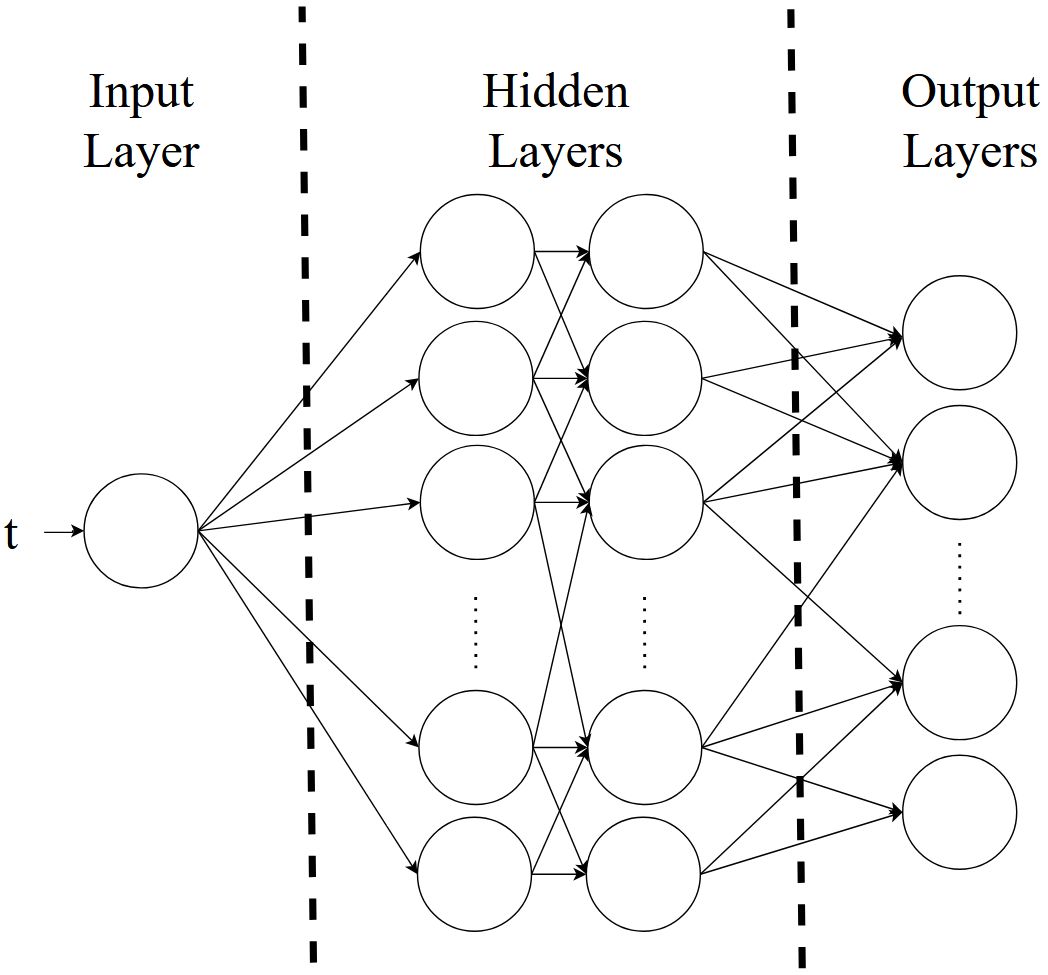
\includegraphics[width=0.3\textwidth]{images/pinns_architecture.png} 
    \caption{Architecture of PINNs and the Multi-agent centralized control systems}
    \label{fig:pinns_and_control_diagram} 
\end{figure}

The MAS we implement is a centeralized control commanding the drones by giving the control input $\boldsymbol{\tau} = [F_B, M_{xB}, M_{yB}, M_{zB}]^T$ relates to individual thrust inputs $\mathbf{u} = [F_1, F_2, F_3, F_4]^T$ via the allocation matrix $A \in \mathbb{R}^{4 \times 4}$:

\begin{equation} \label{eq:tau}
    \boldsymbol{\tau} = [F_B, M_{xB}, M_{yB}, M_{zB}]^T = A \mathbf{u}
\end{equation}
\begin{equation}
    A =
    \begin{bmatrix}
        1 & 1 & 1 & 1 \\
        y_1 & y_2 & y_3 & y_4 \\
        -x_1 & -x_2 & -x_3 & -x_4 \\
        c_1 & c_2 & c_3 & c_4
    \end{bmatrix}
\end{equation}
The rows of $A$ denote total thrust, roll moment, pitch moment, and yaw reactive torque, respectively. Required individual thrusts are derived by inversion:
\begin{equation}
    \mathbf{u} = A^{-1}
    \begin{bmatrix} F_B \ M_{xB} \ M_{yB} \ M_{zB}
    \end{bmatrix}\label{eq:inverse_allocation}
\end{equation}

\subsection{Centralized Control Design}
Based on \cite{mellinger2013trajectory}, the controller separates position and attitude tracking. Position and velocity errors define commanded acceleration $\mathbf{\ddot{r}}_{cmd}$:
\begin{equation}
    \mathbf{e}_p = \mathbf{r}_{des} - \mathbf{r}, \quad \mathbf{e}_v = \mathbf{\dot{r}}_{des} - \mathbf{\dot{r}}
\end{equation}
\begin{equation}\mathbf{\ddot{r}}_{cmd} = K_p \mathbf{e}_p + K_d \mathbf{e}_v + \mathbf{\ddot{r}}_{\text{ff}}
\end{equation}
Desired roll ($\phi^{des}$), pitch ($\theta^{des}$), and total thrust ($F_B^{des}$) are extracted via small-angle approximation:
\begin{equation}
    \begin{split}
        \phi^{des} &= \frac{1}{g} (\ddot{r}^{des}_{x} \sin \psi_T - \ddot{r}^{des}_{y} \cos \psi_T) \\
        \theta^{des} &= \frac{1}{g} (\ddot{r}^{des}_{y} \cos \psi_T + \ddot{r}^{des}_{y} \sin \psi_T) \\
        F_B^{des} &= m(\ddot{r}^{des}_{z} + g)
    \end{split}
\end{equation}
Inner-loop desired moments $\mathbf{M}_B^{des}$ regulate orientation against angular velocities $(p, q, r)$:
\begin{equation}
    \begin{split}        
        M_{xB}^{des} &= k_{p, \phi} (\phi^{des} - \phi) + k_{d, \phi} (p^{des} - p) \\
        M_{yB}^{des} &= k_{p, \theta} (\theta^{des} - \theta) + k_{d, \theta} (q^{des} - q) \\
        M_{zB}^{des} &= k_{p, \psi} (\psi^{des} - \psi) + k_{d, \psi} (r^{des} - r)
    \end{split}
\end{equation}

\subsection{Dynamic Thrust Allocation}
An asymmetric payload shifts the CoG, altering the effective moment arms. Let $\hat{\mathbf{d}}_{\text{cog}} = [\hat{x}_{\text{cog}}, \hat{y}_{\text{cog}}]^T$ denote the estimated offset. Redefining the lever arms as $\Delta x_i = x_i - \hat{x}_{\text{cog}}$ and $\Delta y_i = y_i - \hat{y}_{\text{cog}}$, the allocation matrix adapts dynamically:
\begin{equation}
    A_{\text{final}} = \begin{bmatrix}
    1 & 1 & 1 & 1 \\
    \Delta y_1 & \Delta y_2 & \Delta y_3 & \Delta y_4 \\
    -\Delta x_1 & -\Delta x_2 & -\Delta x_3 & -\Delta x_4 \\
    c_1 & c_2 & c_3 & c_4
    \end{bmatrix} \label{eq:allocation_matrix}
\end{equation}
Control inputs are computed via the Moore-Penrose pseudo-inverse to handle transient rank deficiencies:
\begin{equation}
    \mathbf{u} = A_{\text{final}}^{+} \boldsymbol{\tau}\label{eq:final_u}
\end{equation}

% ------------------------------------------------------------------
% Methodology
% ------------------------------------------------------------------
\section{Estimator Design}
\subsection{PINN Architecture}
To address 6-DOF dynamics, our PINN framework \cite{lakshminarayana_application_2022, mojgani_kolmogorov_2023, raissi_physics-informed_2019} uses time $t$ to solve time-dependent ODEs. Minimizing physics-induced residuals allows the network to identify payload parameters and feed them back into the allocation matrix (Fig.~\ref{fig:pinns_and_control_diagram} and \ref{fig:pinns_architecture}).

\begin{figure}[htbp] 
    \centering 
    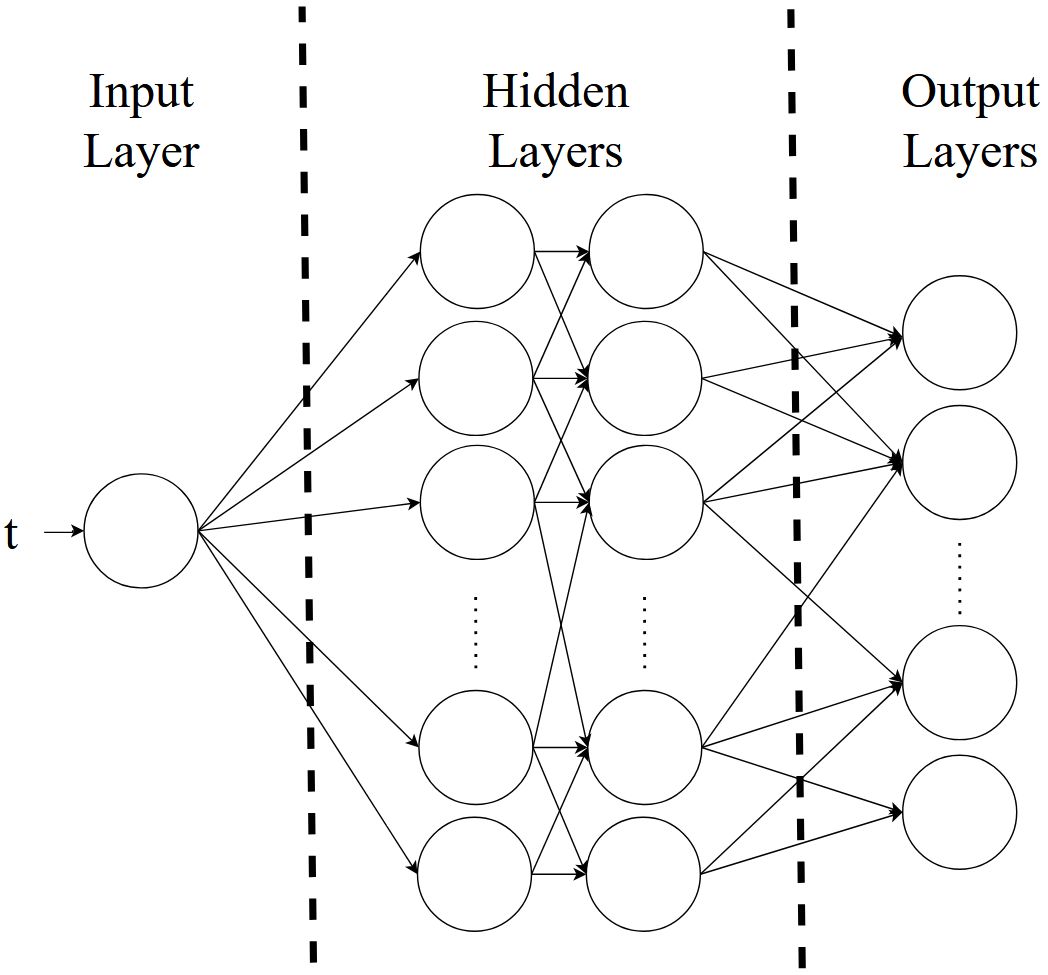
\includegraphics[width=0.3\textwidth]{images/pinns_architecture.png} 
    \caption{Illustration of the PINNs Architecture}
    \label{fig:pinns_architecture} 
\end{figure}

\subsection{Loss Function Formulation}
The system state is $\mathbf{S} = [\mathbf{r}^T, \mathbf{\dot{r}}^T, \boldsymbol{\eta}^T, \boldsymbol{\omega}^T]^T$. The total loss $\mathcal{L}_{total}$ \cite{serrano_physics-informed_2024, raissi_physics-informed_2019} combines data ($\mathcal{L}_{data}$), translational ($\mathcal{L}_{trans}$), and rotational ($\mathcal{L}_{rot}$) residuals:
\begin{equation}
    \mathcal{L}_{total} = \lambda_{1} \mathcal{L}_{data} + \lambda_{2} \mathcal{L}_{trans} + \lambda_{3} \mathcal{L}_{rot} \label{eq:loss_function}
\end{equation}
\begin{equation}
    \mathcal{L}_{data} = \frac{1}{N} \sum_{i=1}^{N} \left\lVert \mathbf{\hat{S}}_i - \mathbf{S}_{true,i} \right\rVert^2 \label{eq:data_loss}
\end{equation}
Translational constraints rely on Euler-Lagrange dynamics:
\begin{equation}
    \frac{d}{dt} \left( \frac{\partial L}{\partial \mathbf{v}} \right) - \frac{\partial L}{\partial \mathbf{r}} = \mathbf{F}_{ext}
\end{equation}
Using PyTorch Autograd for the potential gradient, the residual over $N$ points is:
\begin{equation}
    \mathcal{L}_{trans} = \frac{1}{N} \sum_{i=1}^{N} \left\lVert m \mathbf{\dot{v}}_i + \frac{\partial V}{\partial \mathbf{r}_i} - \mathbf{F}_{ext, i} \right\rVert^2 \label{eq:trans_loss}
\end{equation}
To prevent gimbal lock, rotational dynamics are evaluated on $SO(3)$:
\begin{equation}
    T_{rot} = \frac{1}{2} \boldsymbol{\omega}^T \mathbf{J} \boldsymbol{\omega}
\end{equation}
Applying the Lagrange-d'Alembert principle yields the Euler-Poincaré equations:
\begin{equation}
    \frac{d}{dt} \left( \frac{\partial T_{rot}}{\partial \boldsymbol{\omega}} \right) + \boldsymbol{\omega} \times \frac{\partial T_{rot}}{\partial \boldsymbol{\omega}} = \boldsymbol{\tau}_{ext} \label{eq:euler_poincare}
\end{equation}
Accounting for applied ($\boldsymbol{\tau}_{app}$) and disturbance ($\boldsymbol{\tau}_{dist}$) torques, the rotational residual and resulting loss are:
\begin{equation}
    \text{Res}_{rot} = \left( \mathbf{\hat{J}} \mathbf{\dot{\hat{\boldsymbol{\omega}}}} + \boldsymbol{\hat{\omega}} \times (\mathbf{\hat{J}} \boldsymbol{\hat{\omega}}) \right) - \left( \boldsymbol{\tau}_{app} - \boldsymbol{\tau}_{dist} \right)
\end{equation}
\begin{equation}
    \mathcal{L}_{rot} = \frac{1}{N} \sum_{i=1}^{N} \left\lVert \text{Res}_{rot, i} \right\rVert^2 \label{eq:rot_loss}
\end{equation}

% ------------------------------------------------------------------
% Experiments
% ------------------------------------------------------------------
\section{Simulation and Results}

\subsection{Simulation Environment and Setup}
Simulations were executed in PyBullet at $\Delta t = 1/240$ s (240 Hz). Quadrotor thrust is capped at 50 N, and gravity is $g = 9.81$ m/s$^2$. The unladen frame mass is $m_f = 6.8$ kg, carrying a $m_p = 1.0$ kg payload ($m_{tot} = 7.8$ kg). Each 60-second episode initializes with a uniformly sampled CoG offset:
\begin{equation}
    d_{x, cog}, d_{y, cog} \sim \mathcal{U}(-0.15, 0.15) \text{ meters}
\end{equation}
Flights exceeding a 2.0 m Euclidean distance error are terminated.

\subsection{Simulation Loop}
The Software-in-the-Loop (SITL) architecture interleaves a 240 Hz geometric attitude controller with a 30 Hz PINN estimator, detailed in Algorithm \ref{alg:simulation_loop}.

\begin{algorithm}[htbp]
\caption{Simulation Loop with Control and Online Parameters Estimation}
\label{alg:simulation_loop}
\begin{algorithmic}[1]
\Require Episode maximum $E_{max}$
\Require Simulation duration $T_{max}$, Physics time step $\Delta t$
\Require PINN update interval $N = 8$ (approx. 30 Hz)
\Require Replay buffer $\mathcal{B}$ with capacity $W = 50$
\Require Initial parameter guesses: $\hat{d}_{x}, \hat{d}_{y}, \hat{\mathbf{J}}, \hat{m}$

\State Init current episode $e_{now}$

\While{$e_{now} \le E_{max}$}
    \State Initi quadrotor states $\mathbf{x}_0$
    \State Initi PINN $\mathcal{N}_\theta$ with random weights $\theta$
    \State Simulation time $t \gets 0$
    \State Step counter $k \gets 0$

    \While{$t \le T_{max}$}
        \State Compute target states $\mathbf{p}_d, \mathbf{v}_d, \mathbf{a}_d, \psi_d, \dot{\psi}_d$ at $t$

        \State Current state $\mathbf{x}_k = (\mathbf{p}, \mathbf{v}, \mathbf{R}, \boldsymbol{\omega})$
        \State Append $\mathbf{x}_k$ and rotor thrusts $\mathbf{T}_k$ to buffer $\mathcal{B}$

        \If{$k \pmod N == 0$ \textbf{and} $|\mathcal{B}| == W$}
        \State Compute composite loss $\mathcal{L}_{total}$ over $\mathcal{B}$
        \State Optimize $\theta$
        \State Extract parameters $\hat{d}_{x}, \hat{d}_{y}, \hat{\mathbf{J}}, \hat{m}$ from $\mathcal{N}_\theta$
        \EndIf

        \State Calculate desired $\mathbf{F}_{des}, \mathbf{M}_{des}$
        \State Construct $\mathbf{A}_{\text{final}}$ for offsets $\hat{d}_{x}, \hat{d}_{y}$
        \State Quadrotors commands $\mathbf{u} \gets \mathbf{A}_{\text{final}}^{-1} [\mathbf{F}_{des}^T, \mathbf{M}_{des}^T]^T$

        \State Apply saturated commands $\mathbf{u}$ to physics engine
        \State $t \gets t + \Delta t$
        \State $k \gets k + 1$
    \EndWhile
\EndWhile
\end{algorithmic}
\end{algorithm}

\subsection{Optimization Parameters}
The PINN utilizes a receding horizon buffer of $W = 50$ transitions, executing 3 gradient optimization steps every 5 simulation iterations (Table~\ref{tab:sim_parameters}).

\begin{table}[htbp]
    \centering
    \caption{System and Simulation Parameters}
    \label{tab:sim_parameters}
    \begin{tabular}{lcc}
        \hline
        \textbf{Parameter} & \textbf{Symbol} & \textbf{Value} \\
        \hline
        Simulation/Control Rate & $f$ & 240 Hz \\
        Simulation Time-Step & $\Delta t$ & $1/240$ s \\
        Simulation Duration & $t_{sim}$ & 60 s \\
        Base Frame Mass & $m_f$ & 6.8 kg \\
        Payload Mass & $m_p$ & 1.0 kg \\
        Total System Mass & $m_{tot}$ & 7.8 kg \\
        Max Thrust per Drone & $T_{max}$ & 50 N \\
        Max Distance Error & $e_{max}$ & 2.0 m \\
        Unknown Payload Offset & $d_{cog}$ & $[-0.15, 0.15]$ m \\
        PINN Window Size & $W$ & 50 steps \\
        Optimization Frequency & $N_{opt}$ & 5 steps \\
        Gradient Steps per Cycle & $S_{grad}$ & 3 steps \\
        \hline
    \end{tabular}
\end{table}

% ------------------------------------------------------------------
% Results and Discussion
% ------------------------------------------------------------------
\section{Results and Discussion}

\begin{figure}[htbp]
    \centering
    \begin{tikzpicture}
        \begin{axis}[
            width=0.98\columnwidth, 
            height=4cm,
            xlabel={Time (s)},
            ylabel={Offset (m)},
            grid=major,
            grid style={dashed, gray!30},
            legend pos=south east,
            legend style={
                font=\footnotesize, 
                cells={anchor=east}
            },
            xmin=0,xmax=90,
            ymin=-.6,
            xtick distance=10,
            axis line style={thick},
            tick style={thick}
        ]
            
            \addplot[
                color=red, 
                line width=1.5pt
            ] table [x=time_sec, y=true_offset_x_m, col sep=comma] {data/flight_data_figure_eight_3d_ep_9.csv};
            \addlegendentry{True}
            
            \addplot[
                color=blue!60!black, 
                line width=1pt, 
                dashed 
            ] table [x=time_sec, y=pred_offset_x_m, col sep=comma] {data/flight_data_figure_eight_3d_ep_9.csv};
            \addlegendentry{Predicted}
            
        \end{axis}
    \end{tikzpicture}
    \caption{Predicted payload offset over-time on X-axis at $10^{th}$ episode}
\end{figure}

\begin{figure}[htbp]
    \centering
    \begin{tikzpicture}
        \begin{axis}[
            width=0.98\columnwidth, 
            height=4cm,
            xlabel={Time (s)},
            ylabel={Offset (m)},
            grid=major,
            grid style={dashed, gray!30},
            legend pos=south east,
            legend style={
                font=\footnotesize, 
                cells={anchor=east}
            },
            xmin=0,xmax=90,
            ymin=-.6,
            xtick distance=10,
            axis line style={thick},
            tick style={thick}
        ]
            
            \addplot[
                color=red, 
                line width=1.5pt
            ] table [x=time_sec, y=true_offset_y_m, col sep=comma] {data/flight_data_figure_eight_3d_ep_9.csv};
            \addlegendentry{True}
            
            \addplot[
                color=blue!60!black, 
                line width=1pt, 
                dashed 
            ] table [x=time_sec, y=pred_offset_y_m, col sep=comma] {data/flight_data_figure_eight_3d_ep_9.csv};
            \addlegendentry{Predicted}
            
        \end{axis}
    \end{tikzpicture}
    \caption{Predicted payload offset over-time on Y-axis at $10^{th}$ episode}
\end{figure}

\begin{figure}[htbp]
    \centering
    \begin{tikzpicture}
        \begin{axis}[
            width=0.98\columnwidth, 
            height=4cm,
            xlabel={Time (s)},
            ylabel={Offset (m)},
            grid=major,
            grid style={dashed, gray!30},
            legend pos=south east,
            legend style={
                font=\footnotesize, 
                cells={anchor=east}
            },
            xmin=0,xmax=90,
            ymin=-.6,
            xtick distance=10,
            axis line style={thick},
            tick style={thick}
        ]
            
            \addplot[
                color=red, 
                line width=1.5pt
            ] table [x=, y=true_offset_y_m, col sep=comma] {data/flight_data_figure_eight_3d_ep_9.csv};
            \addlegendentry{True}
            
            \addplot[
                color=blue!60!black, 
                line width=1pt, 
                dashed 
            ] table [x=time_sec, y=pred_offset_y_m, col sep=comma] {data/flight_data_figure_eight_3d_ep_9.csv};
            \addlegendentry{Predicted}
            
        \end{axis}
    \end{tikzpicture}
    \caption{Predicted payload offset over-time on Y-axis at $10^{th}$ episode}
\end{figure}

\subsection{Parameter Convergence and Estimation}
The PINN effectively minimized the physical rotational residuals defined by the Euler-Poincaré equations. Operating on a $W = 50$ receding horizon, the network consistently identified the static CoG offsets ($d_{x, cog}, d_{y, cog}$) within the initial seconds of flight, mapping disturbance torques to spatial asymmetry without requiring persistent excitation maneuvers.

\subsection{Disturbance Rejection and Trajectory Tracking}
In baseline scenarios lacking PINN compensation, the $1.0$ kg asymmetric payload induced parasitic torques that violated the $e_{max} = 2.0$ m threshold, causing failure. Conversely, the PINN-compensated geometric controller adaptively reallocated thrust distribution. By accounting for the CoG shift, the $SE(3)$ controller maintained steady-state hover and executed dynamic trajectories, maintaining Root Mean Square Errors (RMSE) well within safety bounds.

\section{Conclusion and Future Work}
This paper presented a parameter estimation framework for rigid multi-quadrotor systems utilizing an in-the-loop PINN. By formulating rotational physics losses on the $SO(3)$ manifold via Euler-Poincaré equations, the network avoids gimbal lock and ensures mathematically robust convergence. Integrating this estimator into the geometric allocation matrix allows the system to reject unmodeled disturbance torques and maintain stable tracking without physically canted hardware. Future research will extend this methodology to dynamic underactuated slung loads, incorporating coupled pendulum dynamics into the PINN's physical residuals to dampen dynamic oscillations.

\bibliographystyle{IEEEtran}
\bibliography{references}

\end{document}